

\newglossaryentry{komponente}
{
    name=Komponente,
    description={Eine Komponente beschreibt in der Softwarearchitektur im Allgemeinen ein Teil eines Softwaresystems. Die Definition dieses Begriffs wird in speziellen Frameworks weiter spezifiziert. Bezogen auf das in der Arbeit verwendete EJB-Framework, werden bspw. die Beans als Komponenten betrachtet (vgl. \cite{ejbspec})}
}
\newglossaryentry{artefakt}
{
    name=Artefakt,
    description={Ein Artefakt beschreibt in der Software-Entwicklung die Spezifikation einer physischen Informationseinheit als Ergebnis des Software-Entwicklungsprozesses oder dem Deployment bzw. der Ausführung eines Systems. In der UML Spezifikation 2.1.2 \cite{uml} werden u.a. folgende konkrete Beispiele für Artefakte genannt:
    \begin{itemize}
    \item Dateien in denen Source Code enthalten ist
    \item Skripte
    \item Datenbanktabellen    
    \end{itemize}
    \noindent
    Im Kontext dieser Arbeit sind insbesondere die Dateien, in denen Source Code enthalten ist, allgemein als Artefakt bezeichnet}
}


\newglossaryentry{Engine}
{
    name=Engine,
    description={Eine Engine beschreibt eine Software oder einen Teil einer Software, der für eine spezifische Aufgabe verantwortlich ist (vgl. \cite{pcmag}). Die Aufgabe, die die in der Arbeit beschriebenen Source Engines erfüllen, wird in Abschnitt \ref{sec_tdcs} beschrieben}
}


\newglossaryentry{Interface}
{
    name=Interface,
    description={Ein Interface hat im Allgemeinen eine Übersetzungs- oder Vermittlungsfunktion zwischen gekoppelten Systemen (vgl. \cite{interfaces}). Die Bedeutung des Begriffs in dieser Arbeit bezieht sich jedoch auf den Kontext der objektorientierten Programmierung. In diesem Zusammenhang beschreibt ein Interface die Methoden, die in den Klassen, die dieses Interface erfüllen, vorhanden sein müssen}
}


\newglossaryentry{wrappertype}
{
    name=Wrapper-Typ,
    description={Ein Wrapper-Typ wird in der Programmierung auch als Hüllenklasse oder Adapter bezeichnet und entstammen dem \emph{Adapter-Muster} - einem Strukturmuster aus \cite{gof}. Eine solche Hüllenklasse beschreibt eine Klasse, mit der die Schnittstelle einer anderen Klasse angepasst werden kann. So ist es einem Klienten, welcher eine bestimmte Schnittstelle erwartet, möglich über die Hüllenklassen mit einer Klasse zusammenzuarbeiten, die die erwartete Schnittstelle nicht erfüllt. Die in dieser Arbeit beschriebenen Wrapper-Typen setzen dabei auf die Delegation der Schnittstellen-Anfragen. Das folgende Klassendiagramm zeigt die grundlegende Struktur solcher Wrapper-Typen
\begin{figure}[!h]
\centering
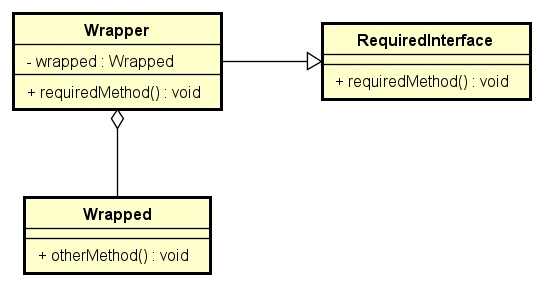
\includegraphics[width=0.75\textwidth]{cd_wrapper.png}
\label{bild}
\end{figure} 
    }
}

\newglossaryentry{JNDI}
{
    name=JNDI,
    description={Java Naming and Directory Interface (JNDI) ist ein API, welches den Entwickler*innen bei der Verwendung der Programmiersprache Java erlaubt, Referenzen von Objekten anhand eines Namens abzulegen und diese Objekte somit auch über den jeweiligen Namen zu adressieren. (vgl. \cite{jndi})}
}

\newglossaryentry{DependencyInjection}
{
    name=Dependency Injection,
    description={Durch Dependency Injection soll die Entkopplung konkreter Implementierungen erreicht werden. Angenommen eine Klasse $A$ hängt von einer Klasse $B$ ab, da sie bspw. ein Attribut vom Typ $B$ enthält. Um die Entkopplung dieser Klassen zu erreichen, wird ein \Gls{Interface} $\mathit{IB}$ geschaffen, welches von der Klasse $B$ implementiert wird. Die Abhängigkeit der zwischen den Klassen $A$ und $B$ wird dann dadurch aufgelöst, dass die Klasse $A$ lediglich vom \Gls{Interface} $BI$. Dieses Vorgehen entspringt dem Paradigma \emph{Inversion of Control} (vgl. \cite{patterns}). Zur Laufzeit muss jedoch dafür gesorgt werden, dass die in einem Objekt der Klasse $A$ ein Objekt injiziert wird, dessen Klasse das Interface $\mathit{IB}$ implementiert - vorzugsweise also ein Objekt der Klasse $B$. Es gibt unterschiedliche Vorgehensweisen, um diese Injektion vorzunehmen (vgl. \cite{setterinjection})}
}

\newglossaryentry{attributgrammatik}
{
    name=Attributgrammatik,
    description={Eine Attributgrammatik ist eine kontextfreie Grammatik, in der die Nonterminale Attribute enthalten können. Dadurch werden die Regeln für die Grammatik um semantische Regeln erweitert, die bestimmen, wie die Attribute der Nonterminale belegt werden müssen. (vgl. \cite{attrGr})}
}

\newglossaryentry{substitutionsprinzip}
{
    name=Substitutionsprinzip,
    description={Das Listkov'sche Substitutionsprinzipt ist ein Entwurfsprinzip der objektorientierten Programmierung. Es besagt, dass ein Unterklasse überall dort einsetzbar sein muss, wo die Oberklasse verlangt wird (vgl. \cite{patterns})}
}

\newacronym{ast}{AST}{\Gls{abstractSyntaxtree}}


\newglossaryentry{abstractSyntaxtree}
{
    name=Abstrakter Syntaxbaum,
    description={Ein abstrakter Syntaxbaum wird für die Darstellung der \emph{abstrakten Syntax} eine Programms verwendet. Diese \emph{abstrakte Syntax} ist eine Datenstruktur, welche die Kerninformationen eines Programms beschreibt, Sie enthält keinerlei Informationen über Details bzgl. der Notation (\emph{konkrete Syntax}). (vgl. \cite{dsl})}
}

\newglossaryentry{downcast}
{
    name=Downcast,
    description={Ein Downcast beschreibt eine Typumwandlung eines Typs $T$ in einen von $T$ abgeleiteten Typen $T'$ ($T > T'$). Zur Laufzeit ergibt sich dabei das Problem, dass in $T'$ eine Methode $m$ deklariert wurde, die jedoch nicht in $T$ bekannt ist. Sofern also ein Objekt vom Typ $T$ dort verwendet wird, wo ein Objekt vom Typ $T'$ erwartet wird, führt der Aufruf der Methode $m$ zwangsweise zu einem Fehler, da die Methode in dem verwendeten Objekt unbekannt ist
}}

\newglossaryentry{Heuristik}
{
    name=Heuristik,
    description={Als Heuristik werden in dieser Arbeit Verfahren bezeichnet, durch die die Lösung eines Problems beschleunigt werden kann, indem neu gewonnene Erkenntnisse bei der Lösungsfindung berücksichtigt werden}
   }

\newglossaryentry{bsort}
{
    name=Bubble-Sort,
    description={Unter dem Bubble-Sort-Verfahren versteht man ein Sortierverfahren, bei dem die Elemente einer Liste, die größer als ihr Nachfolger sind, mit ihrem Nachfolger vertauscht werden. Sofern in der Liste keine Elemente mehr vertauscht werden, gilt die Liste als sortiert
    }
}

\newglossaryentry{Modul}
{
    name=Modul,
    description={Ein Modul ist in der Software-Entwicklung ein Teil eines Softwaresystems, der eine funktional geschlossene Einheit darstellt und einen bestimmten dienst bereitstellt (vgl. \cite{modul}). In dieser Arbeit werden einzelne Java-Projekte als Module bezeichnet}
}

\newglossaryentry{Komplexitaet}
{
    name=Komplexität,
    description={Komplexität wird in dieser Arbeit als Oberbegriff für \Gls{Speicherkomplexitaet} und \Gls{Zeitkomplexitaet} verwendet
    }
}


\newglossaryentry{Speicherkomplexitaet}
{
    name=Speicherkomplexität,
    description={Unter Speicherkomplexität versteht man i.d.R. den Speicherbedarf, den ein Algorithmus benötigt, um ein bestimmtes Problem zu lösen}
}


\newglossaryentry{Zeitkomplexitaet}
{
    name=Zeitkomplexität,
    description={Unter Zeitkomplexität versteht man i.d.R. den Bedarf an Rechenschritten, den ein Algorithmus benötigt, um ein bestimmtes Problem zu lösen}
}

\newglossaryentry{defaultmethode}
{
    name=Default-Methode,
    description={Eine Default-Methode ist eine Methode, die innerhalb eines Java-\Gls{Interface}s implementiert wurde. Sofern diese Methode von den implementierenden Klassen dieses \Gls{Interface}s nicht überschrieben werden, wird beim Aufruf dieser Methode die Implementierung der Default-Methode verwendet (vgl. \cite{dmethod})
    }
}
